\section{Software Design}

This section presents all details about RoboFEI@Home software. A stable version of the software is available on GitHub\footnote{\url{https://github.com/OpenFEI/rfh_judite}}. The section is divided as: (I) Judith's software architecture; (II) face and people recognition; (III) object detection; (IV) speech recognition and synthesis; (V) navigation; (VI) object manipulation.

\subsection{Software Architecture}\label{architecture}
All of Judith's software is developed under Ubuntu Linux 14.04 LTS~\cite{sobell:2014} and ROS Indigo Igloo~\cite{ros:2015}. The initial architecture of Judith is composed by three layers. Each layer is responsible for one part of the code. The first layer receives all data from sensors, extract the features and publish it for AI and Controller nodes (Second Layer). AI and Controller nodes use the features to run algorithms for computer vision, location, planning, pattern recognition, among others. The second layer then sends to the third layer information regarding the movement of the robot, that is, the velocity of the motors, positions or velocity of the manipulator joints and face expressions to display on the iPad. The third layer controls all the actuators drivers and actions. A graphic view of the architecture is presented on Fig.~\ref{fig:architecture}.

\begin{figure}[ht!]
    \centering
    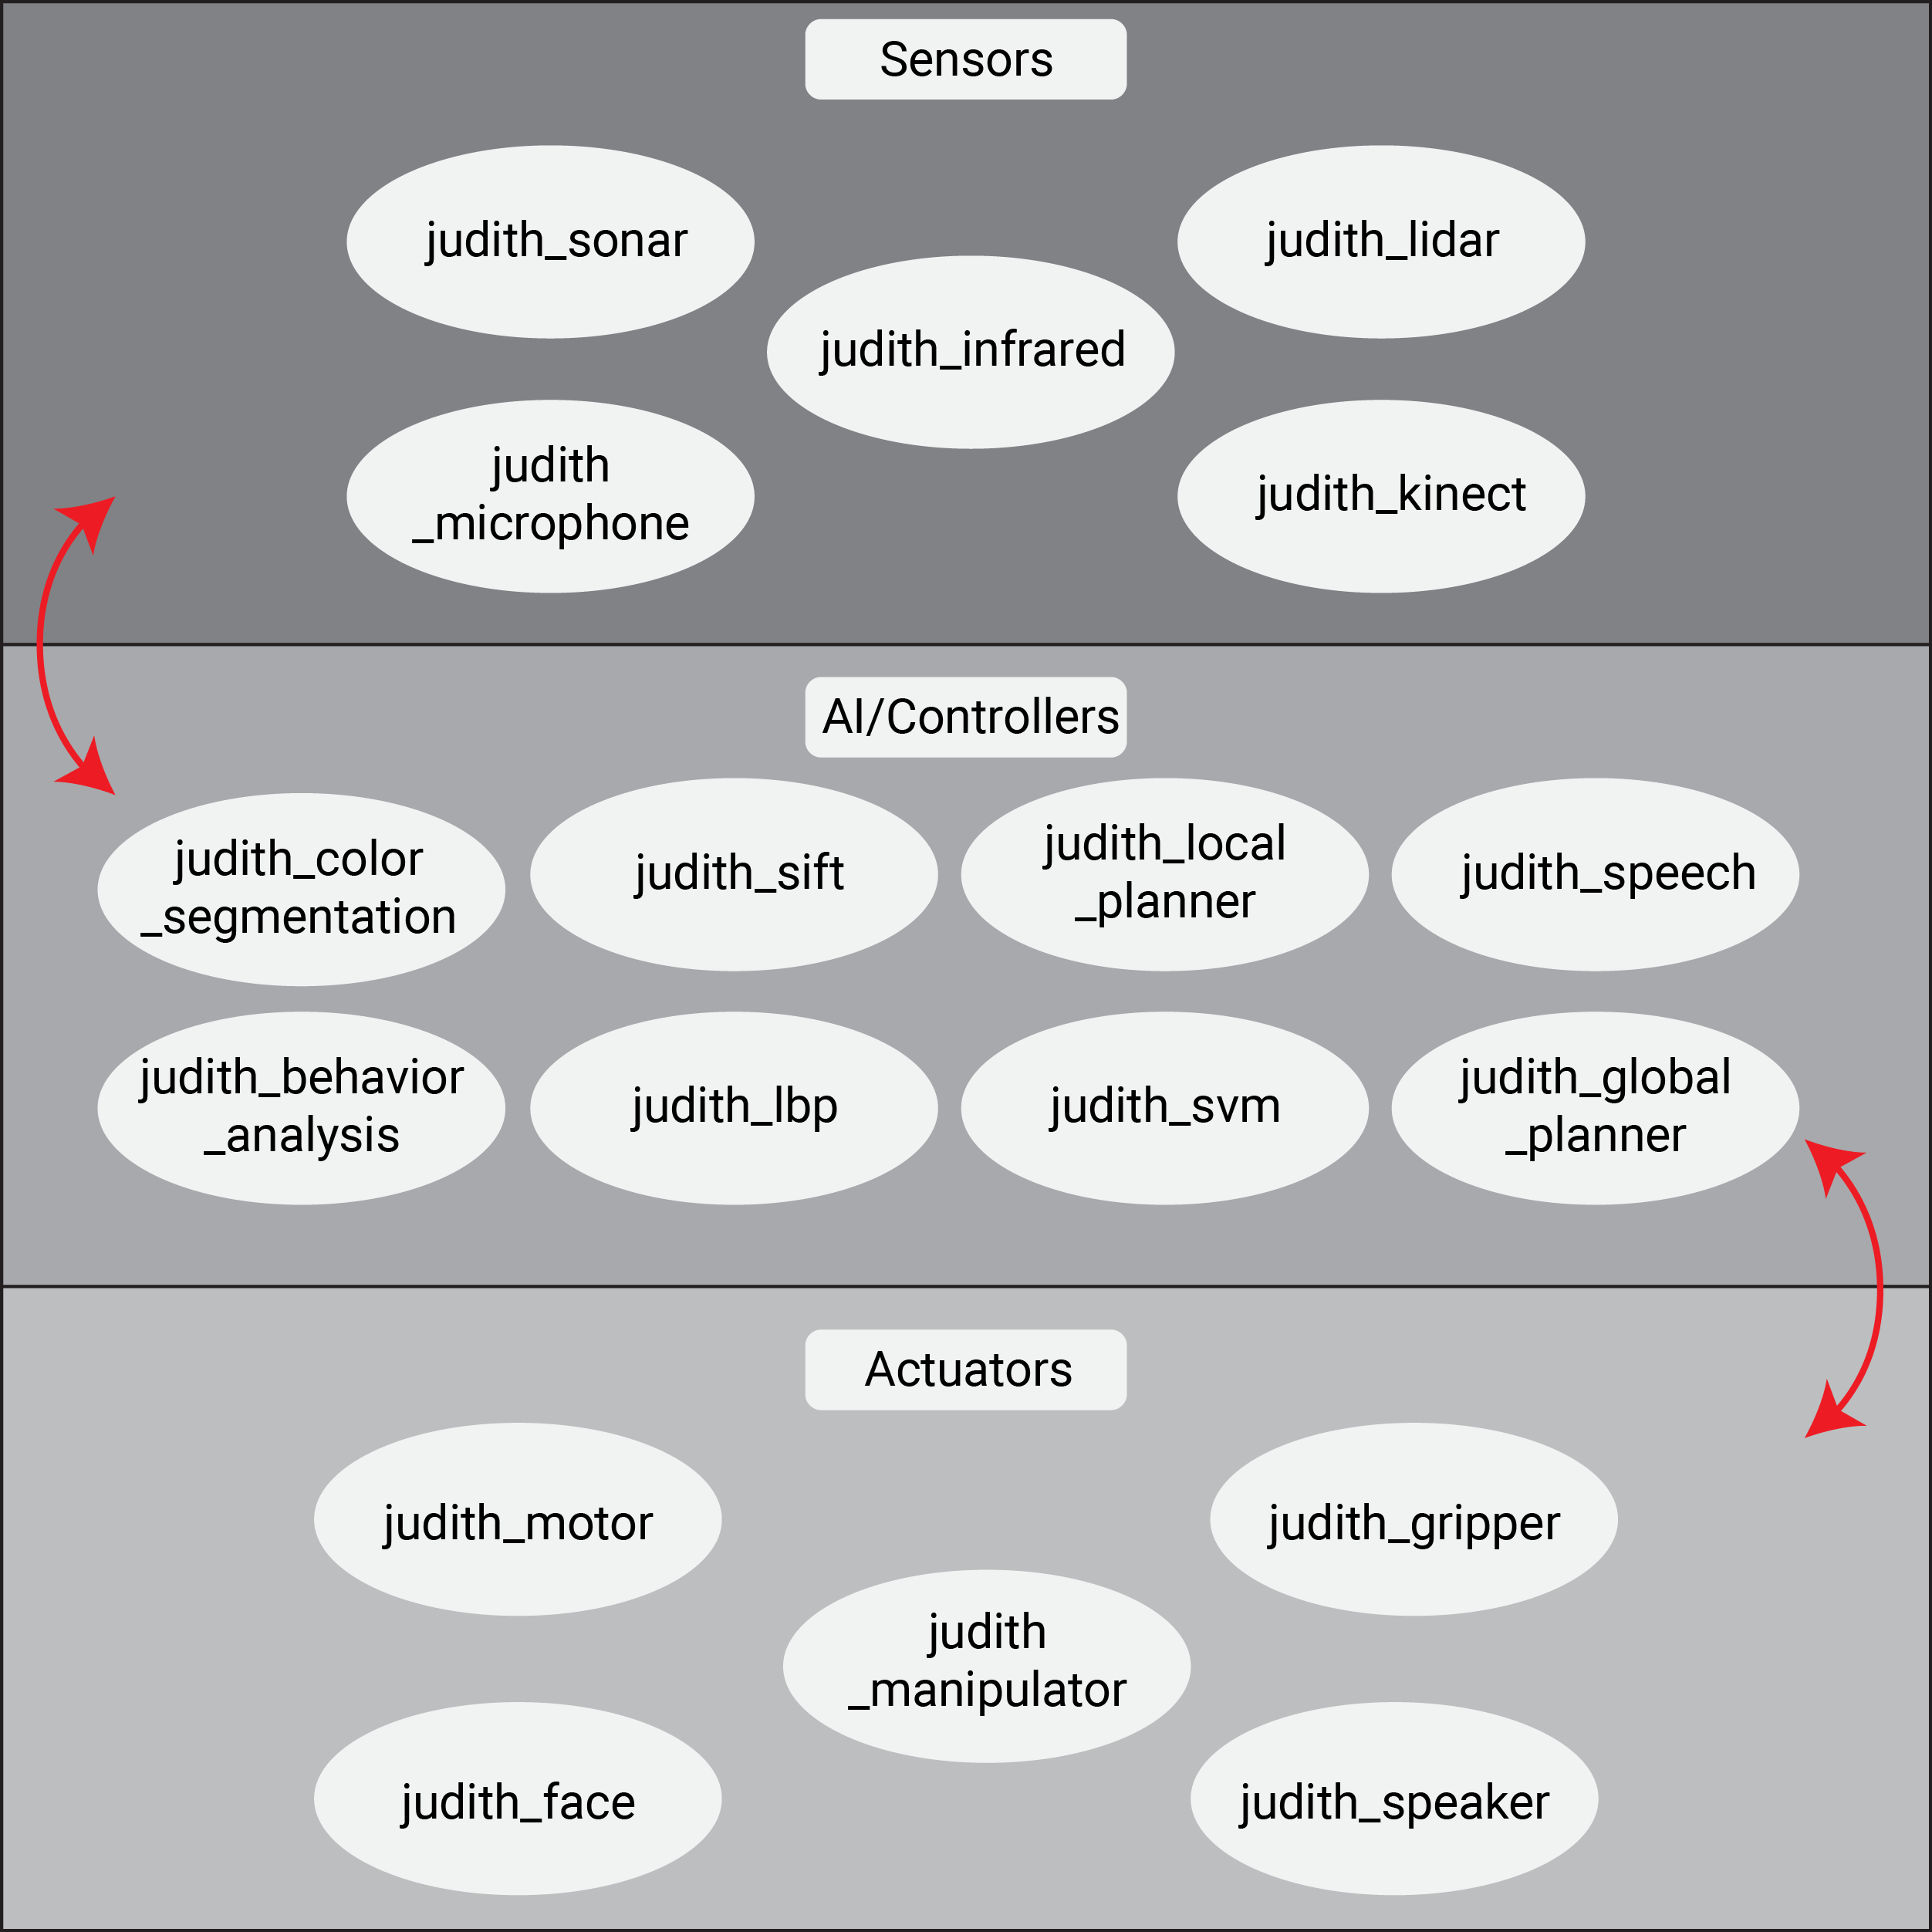
\includegraphics[width = \textwidth]{figures/architecture.png}
    \caption{Software Architecture of Judith}
    \label{fig:architecture}
\end{figure}

Sensors and actuators layers were developed using C++~\cite{stroustrup:1986}, due to hardware drivers communication, except by judith\_face node, which is developed in Java~\cite{joy:2000} language to create an application on Android~\cite{android:2016} Platform. AI/Controllers layer is developed using Python~\cite{vanrossum:2010} as programming language to all algorithms. These decisions were made having in mind the best performance of our robot during task execution and also the training new members to the team.

\subsection{Face and People Recognition}\label{face-people-recognition}
We understand that, in order to make the user's interaction with the robot more comfortable, it is interesting to recognize and treat them by their name. In that way, we developed nodes that can detect and recognize a person by their face. To make it possible, we acquire an image using a camera (Logitech C920 Webcam or Microsoft Kinect X360 RGB camera) and convert the frame into a OpenCV~\cite{bradski:2000} Image Matrix. This information is used as input for the LBP algorithm which has been widely used for face recognition due to its computational performance~\cite{ahonen:2006,yang:2007,shan:2012,ylioinas:2012,samadi:2013}. LBP algorithm may also help on gender, age and facial expression identification which can be useful when developing a robot's adaptive behavior during interaction.

Beyond facial recognition this set of nodes is responsible for following a single person, without external interference during process. To perform this task, three techniques were combined. First is face detection followed by extraction of the color from person t-shirt~\cite{pulli:2012,laganiere:2011,baggio:2012}. With the t-shirt color defined, we perform color segmentation using OpenCV~\cite{kang:2008,oliveira:2009,culjak:2012}. The last technique is skeleton extraction through the Nite/OpenNI library for Microsoft Kinect~\cite{openni:2011}. With this information, the robot can follow the direction of a certain person and also identify the distance between them.

\subsection{Object Detection}\label{object-detection}
Object detection is done by using feature extraction, detection and matching algorithms. A collection of object textures is kept in the robot's memory as bitmap images, each image being part of a class that represents a particular object. When object detection is called for, the robot extracts features from the stored images using either SURF \cite{bay_speeded-up_2008} or SIFT \cite{lowe_object_1999} (the algorithm can be chosen during the robot's startup). Then, it extracts features from the camera feed and matches them with the features from the stored textures. Feature matching is done using brute-force matching: if a certain number of features from a given texture is found in a frame from the camera feed, then a transformation is done to fit the texture in the frame and a rectangle is drawn around the object, identifying it in the frame.

A more efficient object detection procedure is achieved if the robot is able to extract a background image from the environment. The background can be subtracted from frames in real time and object detection is only performed in parts of the frame that change.

\subsection{Speech Recognition and Synthesis}\label{speech}
Speech is one of the most important ways to interact with a human. Because of that, we decided to give Judith a female voice, which is generated by the Festival Speech Synthesis System \footnote{\url{http://www.cstr.ed.ac.uk/projects/festival/}}, developed by the University of Edinburg. Additionally, voice commands are used to start all of the robots functions. Speech recognition is made using the CMU Pocketsphinx~\cite{huggins:2006}.

\subsection{Navigation Stack}\label{navigation}
To interact with the environment, the robot needs to know where it is and how to navigate autonomously. In order to do that, Judith creates a map of the environment using the GMapping application and a Hokuyo URG-04LX-UG01 proximity laser. The map is then saved as a bag using a node from ROS called map\_server. Map generated by GMapping process is presented on figure~\ref{fig:map}.

\begin{figure}[ht!]
    \centering
    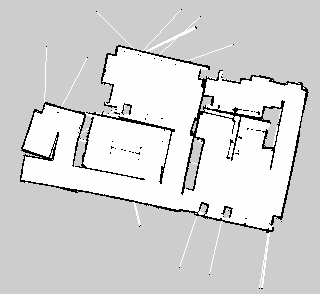
\includegraphics[scale=0.6]{figures/map.png}
    \caption{Map of RoboFEI's Lab}
    \label{fig:map}
\end{figure}

All saved maps can then be used by the robot's simultaneous localization and mapping (SLAM) node. The \emph{Adaptive Monte Carlo Localization} (AMCL) algorithm \cite{fox:1999} uses the maps along with data collected from the laser in real time to make the robot capable to locate its position on the map. With the position known, we are able to give the robot a point to go on the map. It then uses the A* algorithm to make the route between the current position and the desired position. During the completion of the path, it executes a \emph{Dynamic Window Approach}(DWA) algorithm to plan movements locally.

\subsection{Object Manipulation}\label{manipulation}
For manipulating an object, we first use object detection node (see sec.~\ref{object-detection}) to know its current position. The manipulator executes a series of predetermined movements to put the gripper on the robot's view. A PCL algorithm~\cite{aldoma:2012} is then used to segment the gripper and get object distance. In the final step we execute planning to move KUKA youBot arm joints to get the gripper closer and grab the object.
